\section{Résultats}
\subsection{Etude comparative des logiciels bcl2fastq et bcl-convert}
\subsubsection*{Détermination des meilleurs paramètres pour bcl2fastq}
Après avoir effectué différentes combinaisons des paramètres, il a été mis en évidence que la variation du paramètre \texttt{r} et \texttt{w} en fixant le paramètre \texttt{p}, n'apportait pas de différences significatives pour le temps total d'exécution, le temps cpu ou le pourcentage d'utilisation cpu, comme on peut l'observer sur la figure \ref{barplot-param}, pour p fixé à 12. Des resultats similaires ont été obtenus pour p égale à 4, 8 et 16. 

\begin{figure}[H]
    \centering
    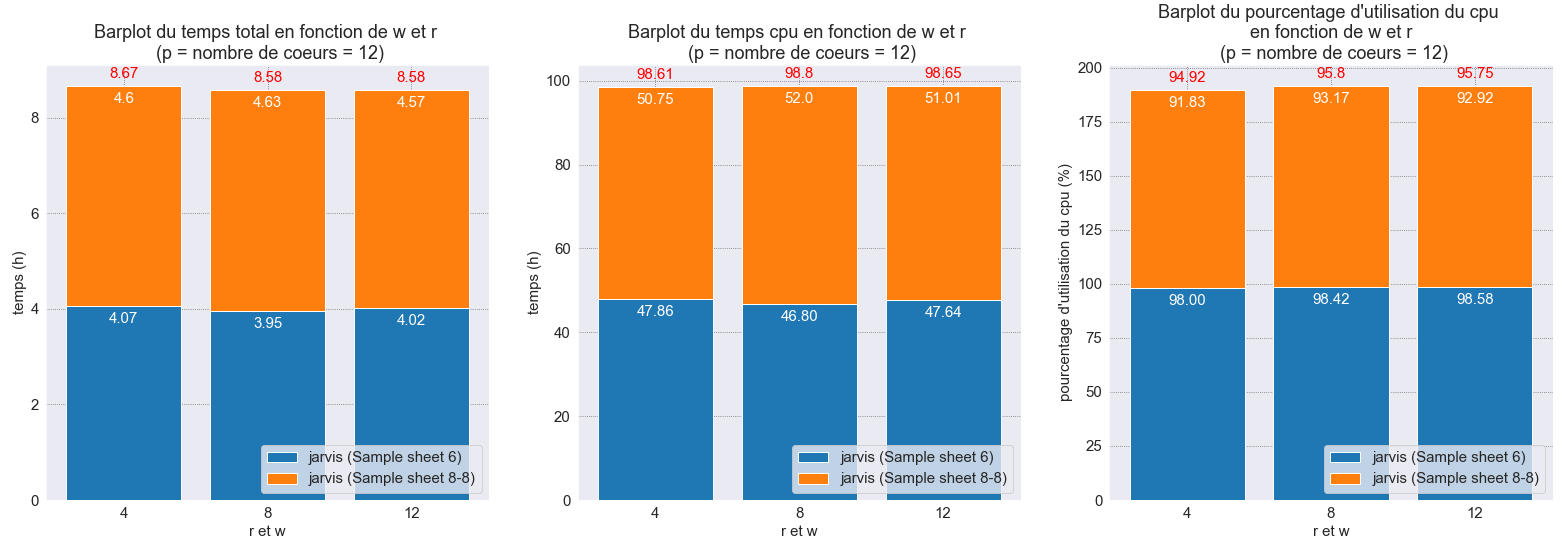
\includegraphics[width=0.8\textwidth]{img/barplot_cum_jarvis2.png}
    \caption{\footnotesize{Digrammes en bâtons du temps total d'éxécution (à gauche), temps cpu (au milieu) et du pourcentage d'utilisation des cpu (à droite) en fonction des paramètres r et w}}
    \label{barplot-param}
\end{figure}

Il y a deux \emph{sample sheet}\footnote{Fichier contenant les informations et instructions pour la génération des FASTQ et le démultipléxage}, car le nombre de bases considérées des index\footnote{Séquence d'une dizaines de nucléotides en amont du primer de la séquence d'ADN à séquencer, permmettant de séparer les séquences de plusieurs échantillons sur une même piste de la flowcell (démultiplxage)} entre les pistes est différent, obligeant à réaliser deux appels différents au logiciel pour générer les FASTQ et le démultipléxage. Ci-dessous, la figure \ref{barplot-param2}, représente les résultats obtenus en faisant varier p et en fixant les paramètres r et w à 4 (ces deux paramètres sont fixés à 4 pour pouvoir comparer les résultats). On observe que plus on augmente le nombre de coeurs pour p, plus l'execution est rapide. On observe que le temps cpu augmente bien avec le nombre de coeurs et que le pourcentage d'utilisation des cpu est optimal (> 90\%).

\begin{figure}[H]
    \centering
    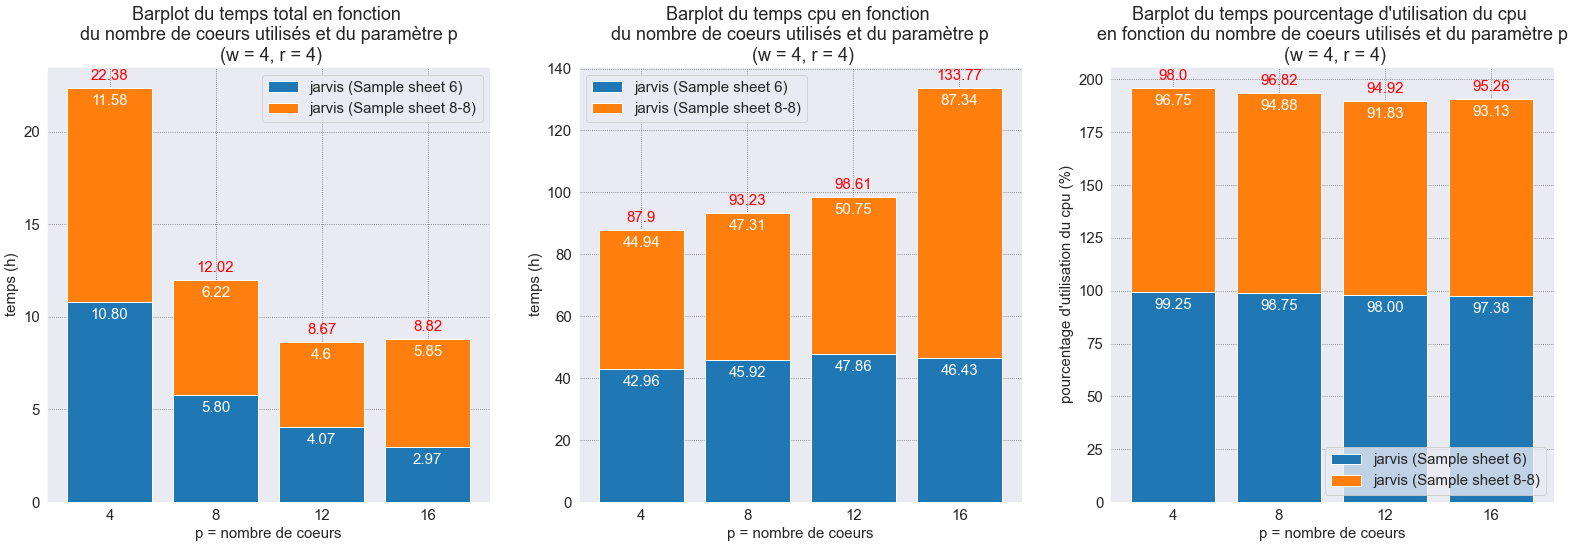
\includegraphics[width=0.8\textwidth]{img/barplot_cum_jarvis1.png}
    \caption{\footnotesize{Digrammes en bâtons du temps total d'éxécution (à gauche), temps cpu (au milieu) et du pourcentage d'utilisation des cpu (à droite) en fonction du paramètre p}}
    \label{barplot-param2}
\end{figure}

Néanmoins, on remarque qu'il n'y a pas d'amélioration du temps total d'execution entre p fixé à 12 et à 16 coeurs. on observe même une augmentation du temps cpu.\\

Au vue des résultats obtenus j'ai décidé que les meilleurs paramètres étaient de fixer p à 12, puisque le gain apporté en augmentant à 16 est faible. Néanmoins j'ai décidé de le conserver pour réaliser la comparaison avec bcl-convert.
Tout comme p fixé à 8, car il nous permettrait de réaliser deux générations de FASTQ et de démultipléxage en simultané sur un seul noeud de calcul de la partition \og production\fg{} puisqu'ils font 16 coeurs.\\

\subsubsection*{Comparaison entre bcl2fastq et bcl-convert}
J'ai donc fait varier les paramètres \texttt{p}, \texttt{r} et \texttt{w} de manière à ce que chacun des paramètre soient égale au nombre de coeurs accordés aux deux logiciels. On observe bien, sur la figure \ref{fig-total-time}, que plus on augmente le nombre de cœurs pour chacun des logiciels, plus la génération des FASTQ et le démultipléxage est rapide. De plus on remarque que bcl-convert permet de réduire le temps d'environs 1/3 par rapport à bcl2fastq. 

\begin{figure}[H]
    \centering
    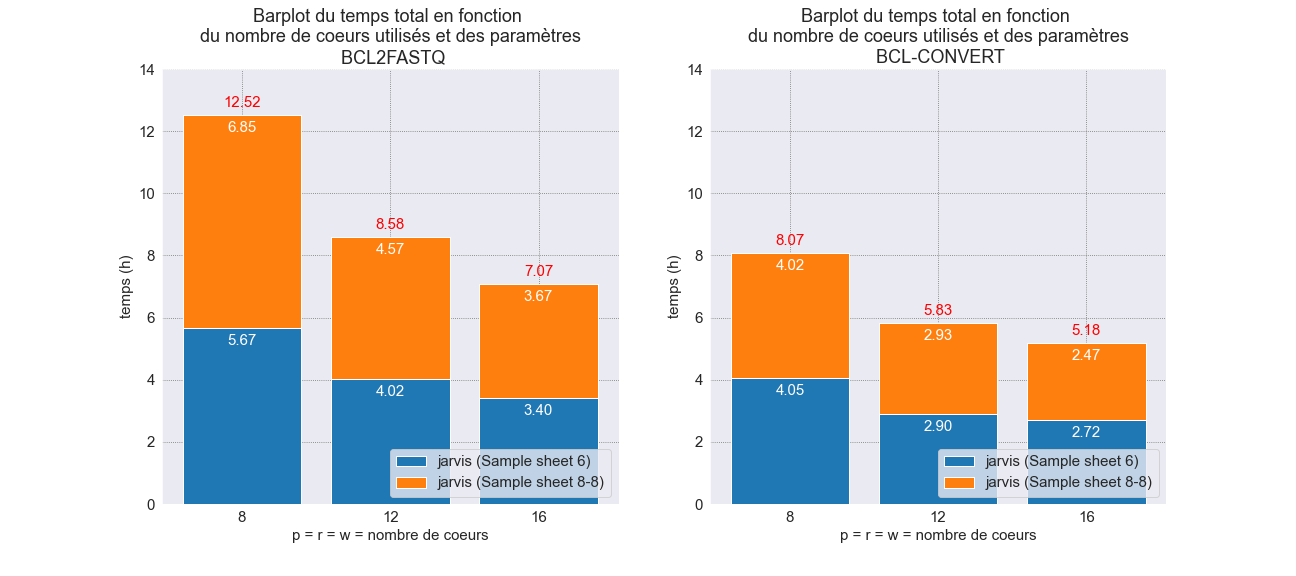
\includegraphics[width=1\textwidth]{img/barplot_total_time_comp.png}
    \caption{\footnotesize{Temps total de génération des FASTQ pour bcl2fastq et bcl-convert}}
    \label{fig-total-time}
\end{figure}

J'ai également échangé avec le service technique d'Illumina à propos des fichiers de sortie et de l'arborescence de ces derniers en utilisant bcl-convert. En effet il s'avère que l'arborescence et les fichiers de sortie sont très différents entre les deux logiciels. Ces échanges avaient pour objectif de savoir si l'on pouvait obtenir une arboresnce similaire à bcl2fastq, pour minimiser l'impact du changement de logiciel sur les pipelines. Le changement de bcl2fastq, qui sera bientôt obsolète, par bcl-convert va donc nous obliger à réaliser de gros changements dans tous les pipelines qui utilisent ces fichiers de sortie.

\subsubsection*{Préparation de la migration de bcl2fastq vers bcl-convert}
Le logiciel bcl-convert est plus rapide d'environ 1/3 par rapport à bcl2fastq. Sachant également que ce dernier sera bientôt obsolète et que le nombre de coeurs disponibles par noeuds pour la partition \og production\fg{} du cluster de calcul est de 16 coeurs, nous avons décidé t'attribuer l'intégralité des coeurs d'un noeud de \og production\fg{}, c'est à dire 16 coeurs et de favoriser le temps d'execution.\\

J'ai consigné l'intégralité des changements entre les deux logiciels dans un cahier des charges. Il contient, la nouvelle commande à lancer, les modules à charger dans l'environement, le chemin relatif des fichiers de sorties et leurs descriptions, ainsi qu'un exemple d'arborescence des fichiers de sorties. Ce qui permettera au développeur qui ce chargera de cette migration de suivre ce cahier des charges et ainsi faciliter cette migration. Dû à la pression actuelle autour de la technologie MGI, c'est un autre développeur de l'équipe, qui sera en charge de réaliser cette migration.

%==============================================================================%
%==============================================================================%

\subsection{Le pipeline de génération de fichiers de séquences pour la technologie MGI}
Le pipeline NGS\_RG\_MGI que j'ai dévellopé à pour objectif de générer et distribuer les fichiers de séquences dans le bon répertoire de projet, d'échantillon, de type de séquençage et de run.
Tout en créant et mettant à jour les runs, pistes et readsets dans NGL\_BI, à l'aide de la librairie Perl permettant d'interagir avec celle-ci (cf. \ref{DBFactory} page \pageref{DBFactory}). Les diférentes etapes du pipeline suivent le schéma (figure \ref{schema-ngsrg-mgi}) que l'on a définit ci-desous.

\begin{figure}[H]
    \centering
    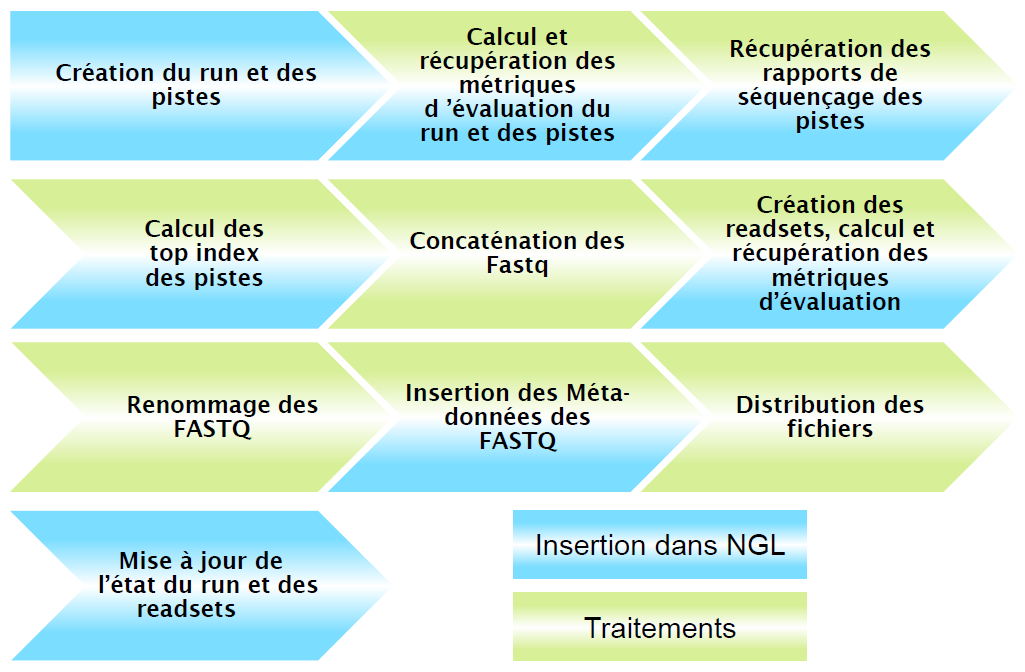
\includegraphics[width=0.8\textwidth]{img/schema-ngsrg-mgi.png}
    \caption{\footnotesize{Schéma des différentes étapes du pipeline NGS\_RG\_MGI. Les étapes qui interagissent avec NGL sont en bleu et les étapes demandant un traitment informatique des données de séquençage sont en vert}}
    \label{schema-ngsrg-mgi}
\end{figure}

\subsubsection*{Création et insertion des métriques du run et des pistes dans NGL }
La première étape du pipeline, que je dévellopé, consite à créer le run et ses pistes dans la base de données NGL, en y insérrant les métriques permettant d'évaluer le run et les pistes (figure \ref{NGL-screenshot_run-lane}).
Le nom du run est constitué de la date de séquençage, du nom du séquenceur et de l'identifiant de la flowcell du run ce qui le rend unique.\\

Les différentes métriques sont insérées à l'aide des librairies Perl permettant d'interagir avec ngl en postant ses métrique dans le fichier JSON du run de la base de données, ce qui permet l'affichage de ces dernières dans l'interface web de NGL\_BI. Toutes ses métriques sont détaillées plus précisement en anexes (page \pageref{anexes1}).\\

\begin{figure}[H]
    \centering
    \fbox{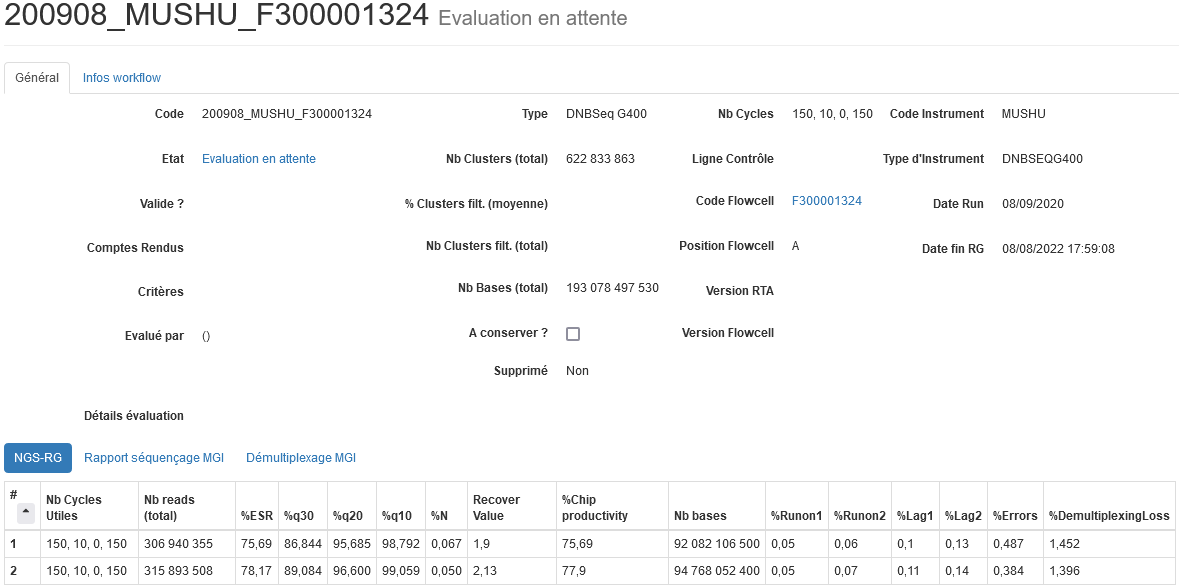
\includegraphics[width=1\textwidth]{img/NGL-screenshot_run-lane-ngsrg.png}}
    \caption{\footnotesize{Capture d'écran de la page du run 200908\_MUSHU\_F300001324 de NGL en cours de génération de fichiers de séquences (étapes d'ajout des métriques d'évaluation du run et des pistes).}}
    \label{NGL-screenshot_run-lane}
\end{figure}

\subsubsection*{Insertion des rapports de séquençage des pistes et de la listes des index dans NGL}
\begin{figure}[H]
    \centering
    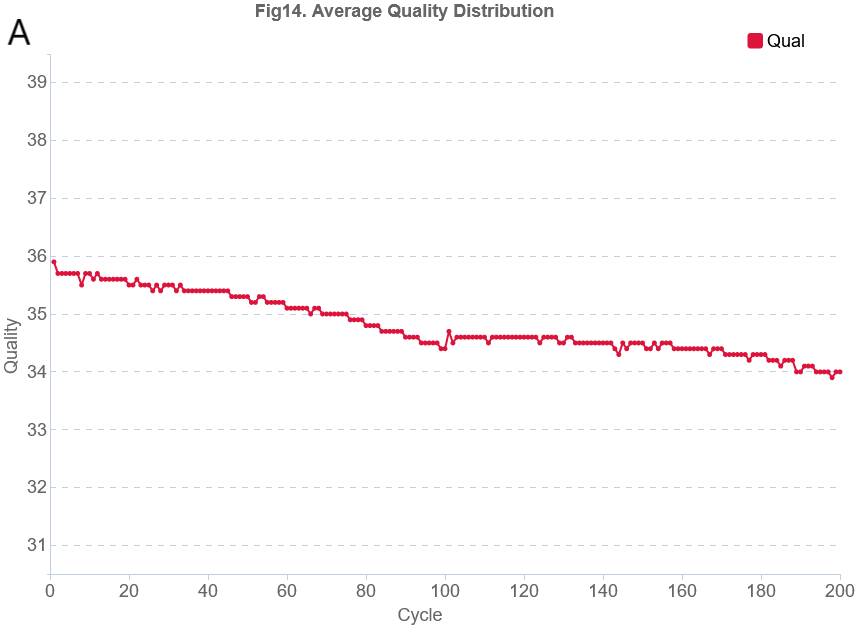
\includegraphics[width=0.45\textwidth]{img/mean_quality.png}
    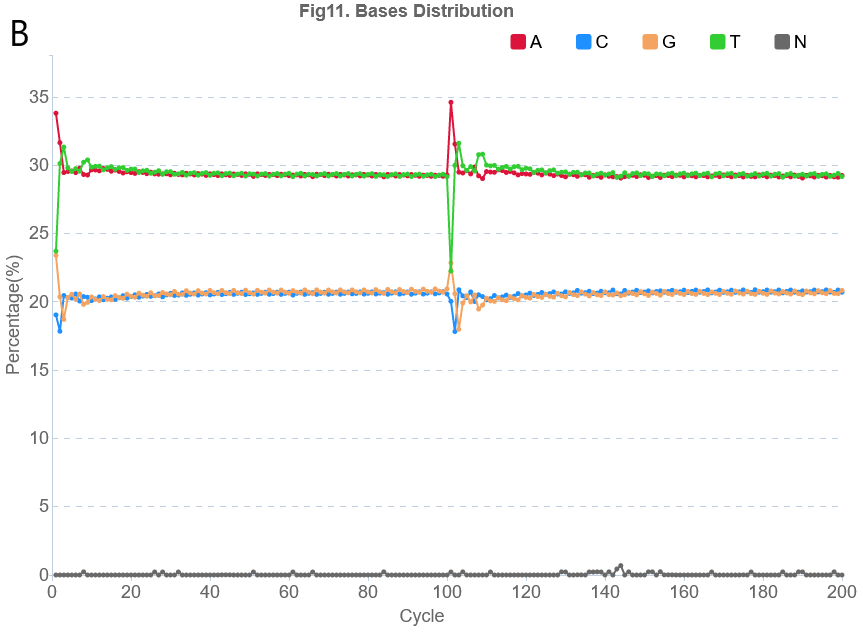
\includegraphics[width=0.45\textwidth]{img/bases_content.png}\\
    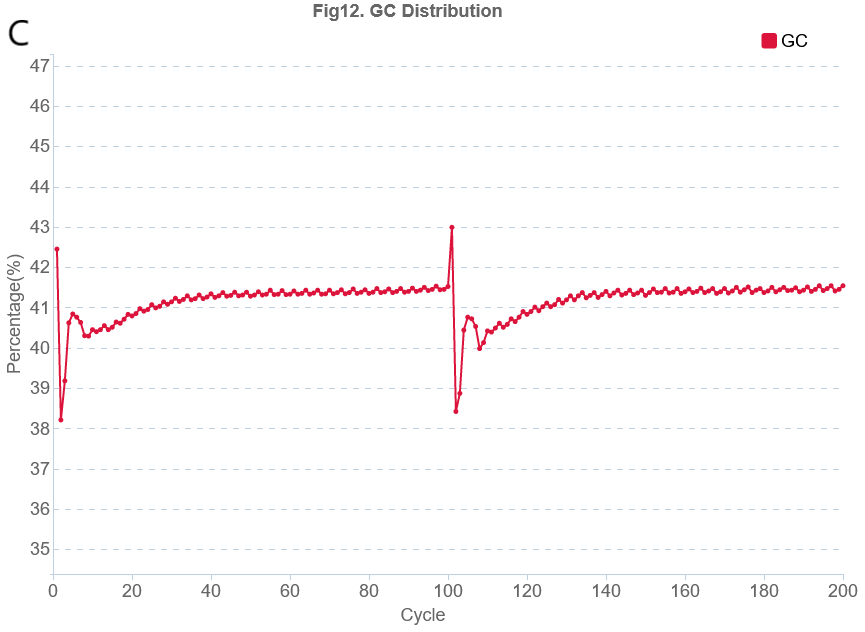
\includegraphics[width=0.45\textwidth]{img/GC_content.png}
    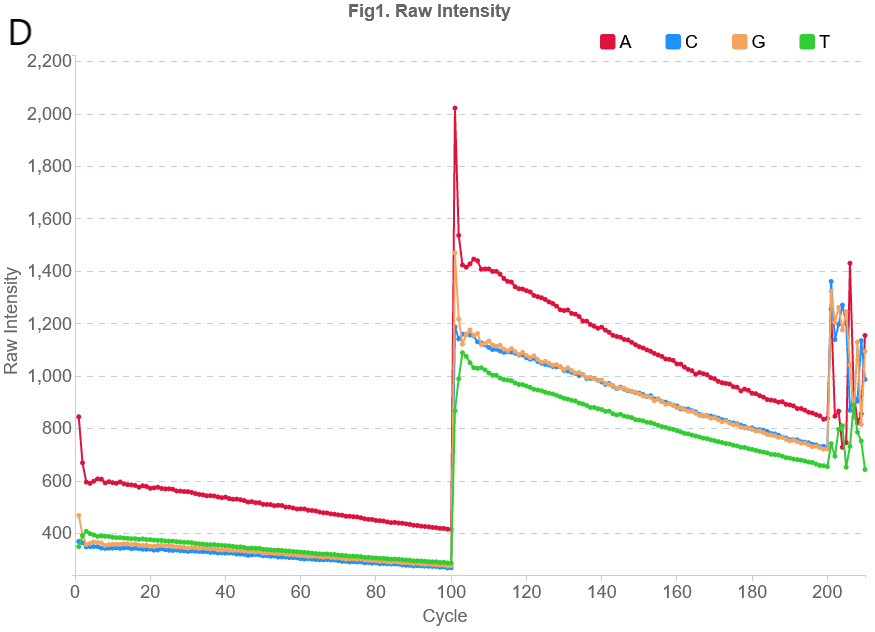
\includegraphics[width=0.45\textwidth]{img/raw_intensity.png}
    \caption{\footnotesize{Graphiques des distributions de la qualité moyenne (A), des bases nucléiques (B), du pourcentage de GC (C) et de l'intensité brut (D) au cours des cycles de séquençage}}
    \label{Graph-rapport-pistes}
\end{figure}

J'ajoute ensuite, en seconde étape, les rapports de séquençage des pistes que le séquenceur génére en fin de séquençage.
Il s'agit de rapports html qui contiennent plusieurs tableaux de métriques et de graphiques permettant d'évaluer les pistes du run.
Il y a notament les graphiques de la distribution de la qualité moyenne en fonction des cycles (figure \ref{Graph-rapport-pistes}\textcolor{blue}{.A}), de la distribution des bases nucléiques en fonction des cycles (figure \ref{Graph-rapport-pistes}\textcolor{blue}{.B}), de la distribution du pourcentage de Guanine/Cytosine en fonction des cycles (figure \ref{Graph-rapport-pistes}\textcolor{blue}{.C}), de la distribution de l'intensité brut au cours des cycles (figure \ref{Graph-rapport-pistes}\textcolor{blue}{.D}).
Les tableaux et graphiques de ces rapports de séquençage permettent de faciliter l'évaluation du run et de ses pistes.\\

Toujours dans l'optique de facilité l'évaluation du run et de ces pistes, l'étape suivante du pipeline, à été  d'ajouter la liste des index représentées à plus de 0.01\% de la piste, ainsi que les index attendus.
Ces index sont triés et affichés par ordre décroissant dans NGL (figure \ref{top-index}).
Les index attendus sont colorés en vert et les index non-attendus ou inconnus sont colorés en rouge, ce qui permet de vérifier que les index attendus sont bien majoritairement représentés sur les pistes de la flowcell du run.

\begin{figure}[H]
    \centering
    \fbox{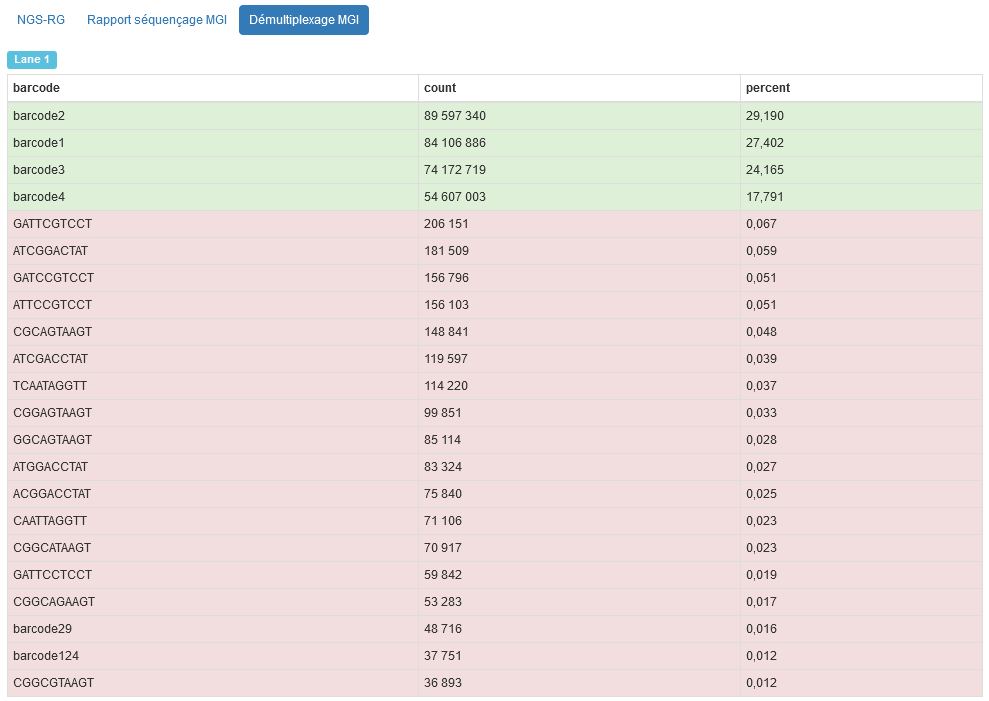
\includegraphics[width=1\textwidth]{img/Top_index.png}}
    \caption{\footnotesize{Capture d'écran de la page du run 200908\_MUSHU\_F300001324 de NGL en cours de génération de fichiers de séquences (onglet \og démultipléxage MGI\fg{})}}
    \label{top-index}
\end{figure}

\subsubsection*{Concaténation des fichiers FASTQ d'un même readset}
Ensuite la quatrième étape du pipeline que j'ai dévellopé à pour objectif d'obtenir un seul fichier FASTQ par readset.
En effet la technologie MGI requiert une homogénéité en composition en base nucléiques (A, T, C, G) au niveau de chaque cycle des index, un déséquilibre étant susceptible d'entraver la récupération du signal pour les bases de ces cycles et donc de fausser leur \emph{base calling} puis le démultipléxage des sequences.
Ainsi il est recommandé de \og barcoder \fg{} les échantillons avec 4 barcodes (index), dont les sequences assurent une composition égale en A, T, C et G à chaque position des barcodes.
Dans ce cas, nous obtenons donc plusieurs fichiers par échantillons qu'il faut donc fusionner pour en obtenir qu'un seul par échantillon lors du démultipléxage effectué par le séquenceur.

Si le readset est associé à un seul readset alors on réalise une décompréssion du fichier FASTQ, à l'inverse si il est associé à plusieurs index on réalise une décompréssion et une concaténation des fichiers FASTQ (cf. figure \ref{schema-concat-fastq}).

\begin{figure}[H]
    \centering
    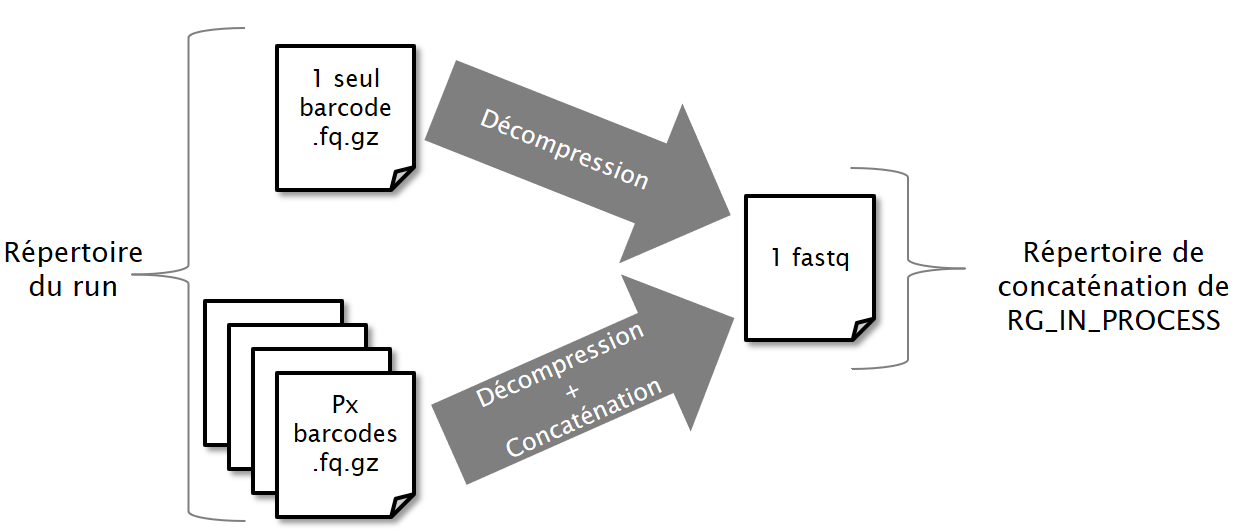
\includegraphics[width=0.8\textwidth]{img/Schéma_concaténation.png}
    \caption{\footnotesize{Schéma de l'étape de \og concaténation\fg{} des fichiers FASTQ d'un readset}}
    \label{schema-concat-fastq}
\end{figure}

\subsubsection*{Création et insertion des métriques des readset du run dans NGL}
La cinquième étape a pour objectif de permettre l'évaluation des readsets, en les créants et en insérant les métriques d'évaluation de ces derniers dans NGL (figure \ref{NGL-screenshot_readset}).
On y retrouve notamment le nombre de bases nucléiques et de reads du readset, ainsi que le pourcentage d'échantillon déposé sur la piste et le pourcentage de séquences valides par rapport au nombre total de séquences de la piste.
J'y insère également certaines métriques du run dont le readset fait partie, comme le nombre de cycles des reads et des index, la date de run, etc. Toutes ces métriques sont décrites en annexes (page \pageref{anexes3})\\

Le nom du readset est constitué de l'identifiant de projet, de l'identifiant du type de banque utilisée (ADN, ARN \dots), de l'identifiant d'échantillon, de l'indice de la piste, de l'identifiant de la flowcell et de l'identifiant du premier barcode ce qui le rend unique également.

\begin{figure}[H]
    \centering
    \fbox{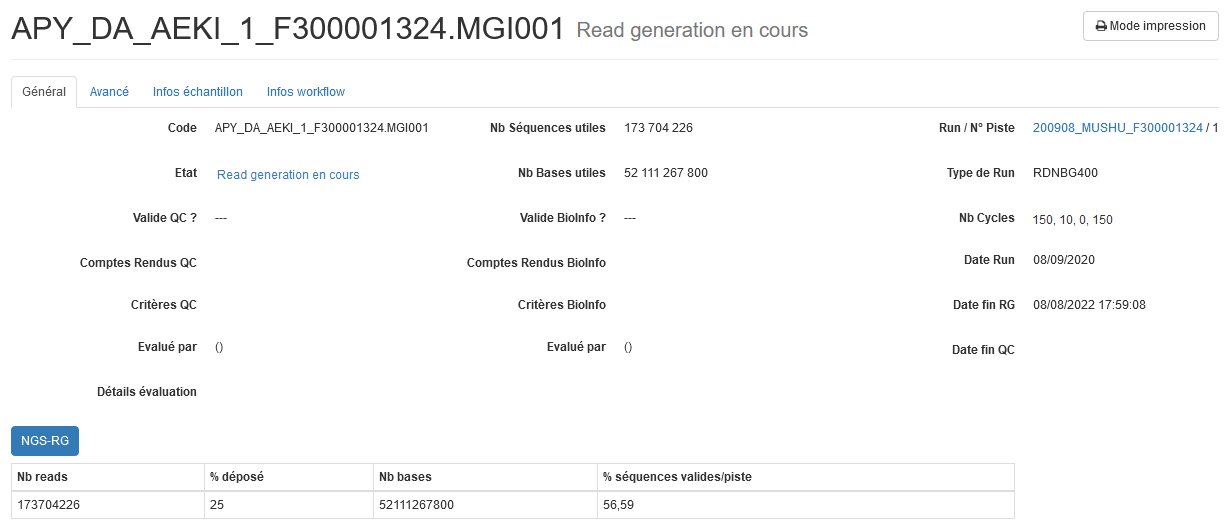
\includegraphics[width=1\textwidth]{img/NGL-screenshot_readset-ngsrg.png}}
    \caption{\footnotesize{Capture d'écran de la page du readset APY\_DA\_AEKI\_1\_F300001324.MGI001 de NGL en cours de génération de reads (étapes de création du readset et d'insertion de ces métriques d'évaluation)}}
    \label{NGL-screenshot_readset}
\end{figure}

L'étape suivante du pipeline est d'ajouter la répartition des index au sein d'un readset (figure \ref{NGL-screenshot_readset-index}), ce qui permet de vérifier la composition en index du readset et de vérifier l'homogénéité de ces index au sein du readset.

\begin{figure}[H]
    \centering
    \fbox{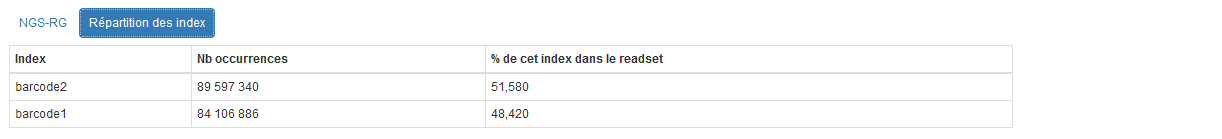
\includegraphics[width=1\textwidth]{img/NGL-screenshot_readset-index.png}}
    \caption{\footnotesize{Capture d'écran de la page du readset APY\_DA\_AEKI\_1\_F300001324.MGI001 de NGL en cours de génération de reads (onglet \og Répartition des index\fg{})}}
    \label{NGL-screenshot_readset-index}
\end{figure}

Au niveaux du run un tableau référençant les readsets et leurs métriques d'évaluation est également ajouté à partir des métriques que j'ai ajouté dans le fichier JSON du readset. (figure \ref{NGL-screenshot_tab-run-readset}).

\begin{figure}[H]
    \centering
    \fbox{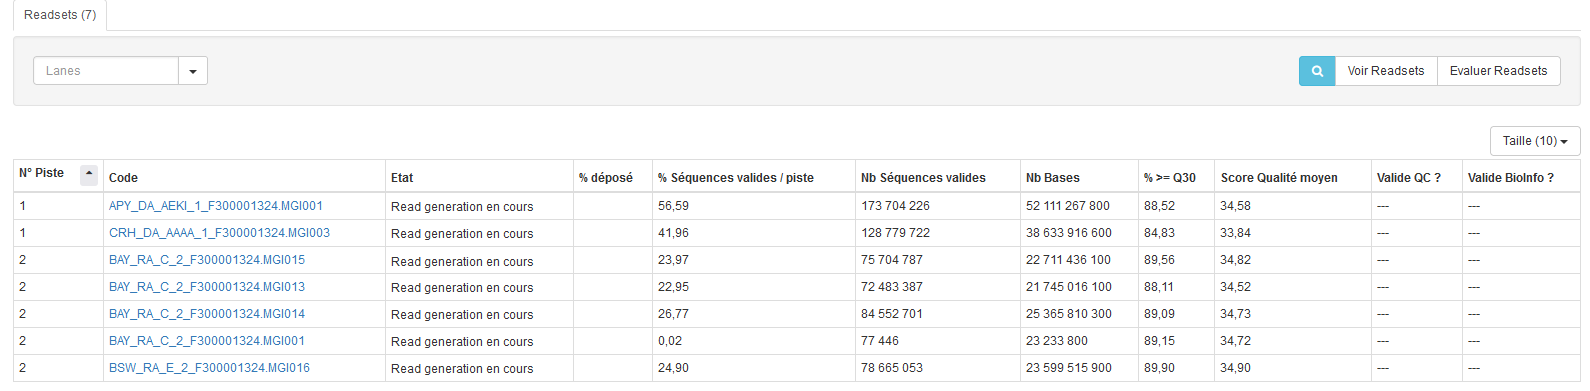
\includegraphics[width=1\textwidth]{img/NGL-screenshot_Tab-readset-in-run.png}}
    \caption{\footnotesize{Capture d'écran de la page du run 200908\_MUSHU\_F300001324 de NGL en cours de génération de fichiers de séquences (Tableau des readset du run)}}
    \label{NGL-screenshot_tab-run-readset}
\end{figure}

\subsubsection*{Renommage des fichiers séquences et insertion des méta-données dans NGL}
La septième étape, consiste à renomer les fichiers de séquences des readsets et d'insérer les méta-données de ces derniers dans NGL via le fichier JSON du readset (figure \ref{meta-data-fastq}).
Le renommage des fichiers est nécessaire pour que chaque fichiers de séquences aient un nom unique et \og parlant\fg{}.\\

\begin{minipage}{0.45\textwidth}
    \begin{figure}[H]
        \centering
        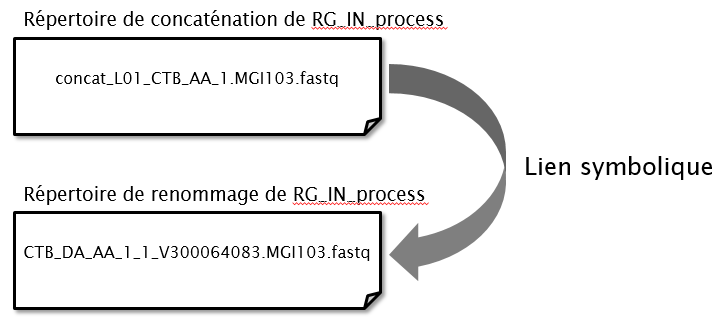
\includegraphics[width=1\textwidth]{img/Schema-renomage-fastq.png}
        \caption{\footnotesize{Schéma de l'étape de renommage des fichiers FASTQ d'un readset}}
        \label{schema-rename-fastq}
    \end{figure}
\end{minipage}
\hfill
\begin{minipage}{0.45\textwidth}
    Le nom doit permettre d'indentifier rapidement et simplement de quel projet, échantillon, flowcell, ect.
    appartienent les fichiers.
    Le renomage des fichiers est effectués en créant un lien symbolique des fichiers obtenus à l'étape de \og concaténation\fg{} dans un répertoire temporaire (cf figure \ref{schema-rename-fastq}).
\end{minipage}\\\\

Les méta-données des fichiers de séquences du readset que j'insére dans NGL permet aux utilisateurs de trouver rapidement l'emplacement de ces derniers sur le système de fichier, le type de fichier qui est disponible (\og raw\fg{}, \og clean\fg{}) et s'ils sont \og utilisable\fg{}, c'est à dire si ils représentent le niveau de qualité maximale disponible pour les échantillons en question.
On y retrouve donc le chemin vers le repertoire de ces fichiers, leurs noms, leurs types, s'ils sont utilisable, s'il s'agit du read \emph{forward} ou \emph{reverse}, et le type d'encodage des valeur de la qualité (Pour les séquenceurs MGI l'encodage est en Phred +33).\\

L'encodage Phred +33, signifie que l'encodage des valeurs de la qualité sont encodées à partir du carractère \og !\fg{}, qui vaut 33 en base 10 dans la table ASCII\footnote{\emph{American Standard Code for Information Interchange} est une norme de l'encodage des caractères} pour une valeurs de qualité de 0. Il y a 42 niveaux de valeurs de qualité, 41 étant le niveau maximale de qualité d'une base nucléique. L'encodage de la qualité en Phred +33, est donc encodé à partir du caractère \og !\fg jusqu'au caractère \og J\fg{}, qui vaut 74 en base 10 dans la table ASCII et représente la valeur maximale de la qualité d'une base.

Un score qualité de 10 indique qu'il y a un probabilité de 90\% que le \emph{base call} soit correct (1 risque sur 10 que la base soit incorrect) et un score de 40 indique une probabilité de 99,99\% que le \emph{base call} soit correct (1 risque sur 10000 que la base soit incorrect).

\begin{figure}[H]
    \centering
    \fbox{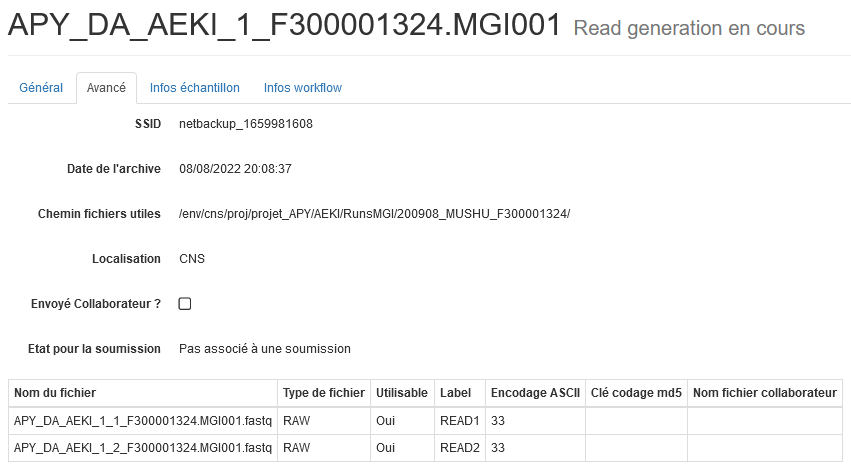
\includegraphics[width=1\textwidth]{img/meta-data-fastq.png}}
    \caption{\footnotesize{Capture d'écran de la page du readset APY\_DA\_AEKI\_1\_F300001324.MGI001 de NGL en cours de génération de fichiers de séquences (Onglet \og Avancé\fg{})}}
    \label{meta-data-fastq}
\end{figure}

\subsubsection*{Distribution des Fichiers séquences et des fichiers de statistiques}
La huitième étape que j'ai dévellopé, permet de distribuer des fichiers de séquences \og attendus\fg{}, les fichiers de statistiques du run et les fichiers de séquences \og non attendus\fg{} dans leurs répertoires dédiés.\\

Les fichiers de séquences \og attendus\fg{} sont copiés vers leur répertoire final en fonction du centre dans lequel le séquençage a eu lieu (Genoscope, CNRGH) et leurs droits d'accès sont modifiés pour que les utilisateurs aient le droit de lecture, mais n'aient pas les droits d'écriture et d'execution.\\

Les fichiers de statistiques du run sont archivés et compressé par pistes et par types (.html, .fq.stat) avant d'être copiés vers leur répertoire final et leurs droits sont changés pour les mêmes raisons .
Ces fichiers sont conservés dans le cas où une métrique désirés ne fait pas partie de celles insérées dans NGL ou pour tout autres problémes qui nécéssiteraient de récupérer les fichiers de statistiques du run.\\

Concernant les fichiers de séquencer \og non attendus \fg{}, il s'agit des fichiers de séquences des index ne faisant pas partie d'un readset. Puisque lors du demultiplexage par les séquenceurs on obtient un fichier FASTQ par index.
Ces fichier sont renomés, archivés, compressés et leurs droits sont changés pour les mêmes raisons que les fichiers de séquences \og attendus\fg{}, avant d'être distribués vers leur répertoire dédiés.
Ces fichers de séquences sont conservés dans l'éventualité d'une mauvaise déclaration d'index par les équipes de séquençages, pour pouvoir récupérer les fichiers fastq appartenant à cet index ou si l'on souhaite étudier les séquences des fichiers \og non-attendus\fg{}.\\

\subsubsection*{Mise à jour de fin de génération de fichiers de séquence dans NGL}
L'étape finale du pipeline de génération de fichiers de séquences pour la technologie MGI, est de mettre à jour le run et les readsets dans l'état de \og F-RG\fg{}, correspondant à la fin du pipeline NGS\_RG.
De plus, les runs n'étant plus dans un état "IW-RG" ou "IP-RG", correspondant à l'attente de prise en charge par NGS\_RG une fois le séquençage terminé ou en cours de génération de reads, ils ne seront plus éligibles à une prise en charge par NGS\_RG.
Cela entraine donc une mise à jour automatique du run à l'état \og IW-V\fg{}, correspondant à l'attente de validation, ce qui permet d'indiquer aux utilisateurs que le run peut être évalué.
Les readsets sont aussi automatiquement mis à jour vers l'état \og IW-QC\fg{}, corespondant à l'attente de prise en charge par le pipeline NGS\_QC, ce qui permette d'indiquer au pipeline de contrôle qualité qu'il peut effectuer le contrôle qualité des readsets de ce run.

